\documentclass[11pt]{amsart}          
\usepackage{amsfonts}
\usepackage{amssymb}  
\usepackage{amsthm} 
\usepackage{amsmath} 
\usepackage{tikz-cd}
\usepackage{float}
\usepackage[]{hyperref}
\usepackage{minted}
\hypersetup{
  colorlinks,
  linkcolor=blue,
  citecolor=blue,
  urlcolor=blue}
\newcommand{\hask}[1]{\mintinline{Haskell}{#1}}
\newenvironment{haskell}
  {\VerbatimEnvironment
  	\begin{minted}[escapeinside=??, mathescape=true,frame=single, framesep=5pt, tabsize=1]{Haskell}}
  {\end{minted}}
 \newcommand*\actL{
  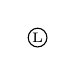
\begin{tikzpicture}[baseline=(C.base)]
    \node[draw,circle,inner sep=0.5pt](C) {\tiny L};
  \end{tikzpicture}}
 \newcommand*\actR{
  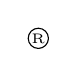
\begin{tikzpicture}[baseline=(C.base)]
    \node[draw,circle,inner sep=0.5pt](C) {\tiny R};
  \end{tikzpicture}}

\author{Bartosz Milewski}
\title{Traversal Optics and Polynomial Functors}

\begin{document}
\maketitle{}

My gateway drug to category theory was the Haskell lens library. What immediately peaked my attention was the van Laarhoven representation, which used functions that are functor-polymorphic. The following function type:
\begin{haskell}
type Lens s t a b = 
  forall f. Functor f => (a -> f b) -> (s -> f t)
\end{haskell}
is isomorphic to the getter/setter pair that traditionally defines a lens:
\begin{haskell}
get :: s -> a
set :: s -> b -> t
\end{haskell}

My intuition was that the Yoneda lemma must be somehow involved. I remember sharing this idea excitedly with Edward Kmett, who was the only expert on category theory I knew. The reasoning was that a polymorphic function in Haskell is equivalent to a natural transformation in category theory. The Yoneda lemma relates natural transformations to functor values. Let me explain.

In Haskell, the Yoneda lemma says that, for any functor \hask{f}, this polymorphic function:
\begin{haskell}
forall x. (a -> x) -> f x
\end{haskell}
is isomorphic to \hask{(f a)}. 
In category theory, one way of writing it is:
\[ \int_{x} \mathbf{Set}\big(\mathcal{C}(a, x), f x\big) \cong f a \]
If this looks a little intimidating, let me go through the notation:
\begin{itemize}
\item The functor $f$ goes from some category $\mathcal{C}$ to the category of sets, which is called $\mathbf{Set}$. Such functor is called a co-presheaf.

\item $\mathcal{C}(a, x)$ stands for the set of arrows from $a$ to $x$ in $\mathcal{C}$, so it corresponds to the Haskell type \hask{a->x}. In category theory it's called a hom-set. The notation for hom-sets is: the name of the category followed by names of two objects in parentheses.

\item $\mathbf{Set}\big(\mathcal{C}(a, x), f x\big)$ stands for a set of functions from $\mathcal{C}(a, x)$ to $f x$ or, in Haskell \hask{ (a -> x)-> f x}. It's a hom-set in $\mathbf{Set}$.
\item Think of the integral sign as the \hask{forall} quantifier. In category theory it's called an \emph{end}. Natural transformations between two functors $f$ and $g$ can be expressed using the end notation:
\[\int_x \mathbf{Set}(f x, g x)\]


\end{itemize}
As you can see, the translation is pretty straightforward. The van Laarhoven representation in this notation reads:
\[ \int_f \mathbf{Set}\big( \mathcal{C}(a, f b), \mathcal{C}(s, f t) \big) \]

If you vary $x$ in $\mathcal{C}(b, x)$, it becomes a functor, which is called a \emph{representable} functor---the object $b$ ``representing'' the whole functor. In Haskell, we call it the reader functor:
\begin{haskell}
newtype Reader b x = Reader (b -> x)
\end{haskell}

You can plug a representable functor it into the Yoneda lemma to get the following very important corollary:
\[ \int_x \mathbf{Set}\big(\mathcal{C}(a, x), \mathcal{C}(b, x)\big) \cong \mathcal{C}(b, a) \]
The set of natural transformation between two representable functors is isomorphic to a hom-set between the representing objects. (Notice that the objects are swapped.)

\section{The van Laarhoven representation}

There is just one little problem: the \hask{forall} quantifier in the van Laarhoven formula goes over functors, not types. 

This is okay, though, because category theory works at many levels. Functors themselves form a category, and the Yoneda lemma works in that category too. 

For instance, the category of functors from $\mathcal{C}$ to $\mathbf{Set}$ is called $[\mathcal{C},\mathbf{Set}]$. A hom-set in that category is a set of natural transformations between two functors which, as we've seen, can be expressed as an end:
\[ [\mathcal{C},\mathbf{Set}](f, g) \cong \int_x \mathbf{Set}(f x, g x) \]
Remember, it's the name of the category, here $ [\mathcal{C},\mathbf{Set}]$, followed by names of two objects (here, functors $f$ and $g$) in parentheses.

So the corollary to the Yoneda lemma in the functor category, after a few renamings, reads:
\[ \int_f \mathbf{Set}\big( [\mathcal{C},\mathbf{Set}](g, f),  [\mathcal{C},\mathbf{Set}](h, f)\big) \cong  [\mathcal{C},\mathbf{Set}](h, g) \]

This is getting closer to the van Laarhoven formula because we have the end over functors, which is equivalent to 
\begin{haskell}
forall f. Functor f => ...
\end{haskell}
In fact, a judicious choice of $g$ and $h$ is all we need to finish the proof.

But sometimes it's easier to define a functor indirectly, as an adjoint to another functor. Adjunctions actually allow us to switch categories. A functor $L$ defined by a mapping-out in one category can be adjoint to another functor $R$ defined by its mapping-in in another category.
\[ \mathcal{C}(L a, b) \cong \mathcal{D}(a, R b) \]
A useful example is the currying adjunction in $\mathbf{Set}$:
\[\mathbf{Set}(c \times a, y) \cong \mathbf{Set}(c, y^a) \cong  \mathbf{Set}\big(c, \mathbf{Set}(a, y)\big) \]
where $y^a$ corresponds to the function type \hask{a->y} and, in $\mathbf{Set}$, is isomorphic to the hom-set $\mathbf{Set}(a, y)$. This is just saying that a function of two arguments is equivalent to a function returning a function.

Here's the clever trick: let's replace $g$ and $h$ in the functorial Yoneda lemma with $L_b a$ and $L_t s$, where $L_b$ and $L_t$ are some higher-order functors from $\mathcal{C}$ to $[\mathcal{C},\mathbf{Set}]$ (as you will see, this notation anticipates the final substitution). We get:
\[ \int_f \mathbf{Set}\big( [\mathcal{C},\mathbf{Set}](L_b a, f),  [\mathcal{C},\mathbf{Set}](L_t s, f)\big) \cong  [\mathcal{C},\mathbf{Set}](L_t s, L_b a) \]
Now suppose that these functors are left adjoint to some other functors: $R_b$ and $R_t$ that go in the opposite direction from $[\mathcal{C},\mathbf{Set}]$ to $\mathcal{C}$ . We can then replace all mappings-out in $ [\mathcal{C},\mathbf{Set}]$ with the corresponding mappings-in in $\mathcal{C}$:
\[ \int_f \mathbf{Set}\big( \mathcal{C}(a, R_b f),  \mathcal{C}(s, R_t f)\big) \cong \mathcal{C}\big(s, R_t (L_b a)\big) \]
We are almost there! The last step is to realize that, in order to get the van Laarhoven formula, we need:
\[R_b f = f b\]
\[R_t f = f t \]
 So these are just functors that apply $f$ to some fixed objects: $b$ and $t$, respectively. The left-hand side becomes:
\[ \int_f \mathbf{Set}\big( \mathcal{C}(a, f b), \mathcal{C}(s, f t) \big) \]
which is exactly the van Laarhoven representation. 

Let's now look at the right-hand side:
\[  \mathcal{C}\big(s, R_t (L_b a)\big) =  \mathcal{C}\big( s, (L_b a) t \big)\]
We know what $R_b$ is, but what's its left adjoint $L_b$? It must satisfy the adjunction:
\[ [\mathcal{C},\mathbf{Set}](L_b a, f) \cong \mathcal{C}(a, R_b f) = \mathcal{C}(a, f b)\]
or, using the end notation:
\[ \int_x \mathbf{Set}\big((L_b a) x, f x\big) \cong \mathcal{C}(a, f b)\]
The identity has a simple solution when  $\mathcal{C}$ is $\mathbf{Set}$, so we'll just temporarily switch to $\mathbf{Set}$. We have:
\[(L_b a) x =  \mathbf{Set}(b, x) \times a \]
which is known as the \hask{IStore} comonad in Haskell. We can check the identity by first applying the currying adjunction to eliminate the product:
\[ \int_x \mathbf{Set}\big(\mathbf{Set}(b, x) \times a, f x\big) \cong \int_x \mathbf{Set}\big(\mathbf{Set}(b, x), \mathbf{Set}(a, f x )\big) \]
and then using the Yoneda lemma to replace $x$ with $b$,
\[ \int_x \mathbf{Set}\big(\mathbf{Set}(b, x), \mathbf{Set}(a, f x )\big) \cong \mathbf{Set}(a, f b)\]
So the right hand side of the original identity, after replacing $\mathcal{C}$ with $\mathbf{Set}$, becomes:
\[  \mathbf{Set}\big(s, R_t (L_b a)\big) \cong \mathbf{Set}\big( s, (L_b a) t \big) \cong \mathbf{Set}\big(s,  \mathbf{Set}(b, t) \times a) \big) \]
which can be translated to Haskell as:
\begin{haskell}
(s -> b -> t, s -> a)
\end{haskell}
or a pair of \hask{set} and \hask{get}.

I was very proud of myself for finding the right chain of substitutions, so I was pretty surprised when I learned from Mauro Jaskelioff and Russell O'Connor that they had a paper ready for publication with exactly the same proof (they added a reference citing my blog post). 

\section{The Existentials}
But there's more: there are other optics for which this trick doesn't work. The simplest one was the prism defined by a pair of functions:
\begin{haskell}
match :: s -> Either t a
build :: b -> t
\end{haskell}
In this form it's hard to see a commonality between a lens and a prism. There is, however, a way to unify them using existential types. 

Here's the idea: A lens can be applied to types that, at least conceptually, can be decomposed into two parts: the focus and the residue. It lets us extract the focus using \hask{get}, and replace it with a new value using \hask{set}, leaving the residue unchanged. 

The important property of the residue is that it's opaque: we don't know how to retrieve it, and we don't know how to modify it. All we know about it is that it \emph{exists} and that it can be combined with the focus. This property can be expressed using existential types. 

Symbolically, we would want to write something like this:
\begin{haskell}
type Lens s t a b = exists c . (s -> (c, a), (c, b) -> t)
\end{haskell}
where \hask{c} is the residue.  We have a pair of functions: The first decomposes the source \hask{s} into the product of the residue \hask{c} and the focus \hask{a} . The second recombines the residue with the new focus \hask{b} resulting in the target \hask{t}.

Existential types can be encoded in Haskell using GADTs:
\begin{haskell}
data Lens s t a b where
  Lens :: (s -> (c, a), (c, b) -> t) -> Lens s t a b
\end{haskell}
They can also be encoded in category theory using coends. So the lens can be written as:
\[ \int^c \mathcal{C}(s, c \times a) \times \mathcal{C}(c \times b, t) \]
The integral sign with the argument at the top is called a coend. You can read it as ``there exists a $c$''.

There is a version of the Yoneda lemma for coends as well:
\[ \int^c f c \times \mathcal{C}(c, a) \cong f a \]
The intuition here is that, given a functorful of $c$'s and a function \hask{c->a}, we can \hask{fmap} the latter over the former to obtain \hask{f a}. We can do it even if we have no idea what the type \hask{c} is.

We can use the currying adjunction and the Yoneda lemma to transform the new definition of the lens to the old one:
\[ \int^c \mathcal{C}(s, c \times a) \times \mathcal{C}(c \times b, t) \cong \int^c \mathcal{C}(s, c \times a) \times \mathcal{C}(c, t^b) \cong \mathcal{C}(s, t^b \times a)\]
The exponential $t^b$ translates to the function type \hask{b->t}, so this this is really the \hask{set}/\hask{get} pair that defines the lens.

The beauty of this representation is that it can be immediately applied to the prism, just by replacing the product with the sum (coproduct). This is the existential representation of a prism:
\[ \int^c \mathcal{C}(s, c + a) \times \mathcal{C}(c + b, t) \]

To recover the standard encoding, we use the mapping-out property of the sum:
\[  \mathcal{C}(c + b, t) \cong  \mathcal{C}(c, t)  \times  \mathcal{C}(b, t) \]
This is simply saying that a function from the sum type is equivalent to a pair of functions---what we call the case analysis in programming.

We get:
\[ \int^c \mathcal{C}(s, c + a) \times \mathcal{C}(c + b, t) \cong \int^c \mathcal{C}(s, c + a) \times \mathcal{C}(c, t)  \times \mathcal{C}(b, t)\]
This has the form suitable for the use of the Yoneda lemma, namely:
\[ \int^c f c \times \mathcal{C}(c, t) \]
with
\[ f c = \mathcal{C}(s, c + a) \times \mathcal{C}(b, t) \]
The result of the Yoneda is replacing $c$ with $t$, so the result is:
\[ \mathcal{C}(s, t + a) \times \mathcal{C}(b, t)\]
which is exactly the \hask{match}/\hask{build} pair (in Haskell, the sum is translated to \hask{Either}).

It turns out that every optic has an existential form.

\section{Double Yoneda}

If you squint hard enough, the Yoneda lemma 
\[ \int_{x} \mathbf{Set}\big(\mathcal{C}(a, x), f x\big) \cong f a \]
could be interpreted as the representable functor $\mathcal{C}(a, -)$ acting as the unit with respect to taking the end. It takes an $f$ and returns an $f$. 

We are going to need an identity that involves a higher-order natural transformation between two higher-order functors. These are actually the functors $R_a$ we've encountered before. They are parameterized by objects in $\mathcal{C}$, and their action on functors (co-presheaves) is to apply those functors to objects. They are the ``give me a functor and I'll apply it to my favorite object'' kind of functors. 

We need a natural transformation between two such functors, and we can express it as an end:
\[ \int_f  \mathbf{Set}( R_a f, R_s f) = \int_f  \mathbf{Set}( f a, f s) \]

Here's the trick: replace these functors with their Yoneda equivalents:
\[ \int_f  \mathbf{Set}( f a, f s) \cong \int_f  \mathbf{Set}\Big(\int_{x} \mathbf{Set}\big(\mathcal{C}(a, x), fx), \int_{y} \mathbf{Set}\big(\mathcal{C}(s, y), f y\big)\Big)\]
Notice that this is now a mapping between two hom-sets in the functor category, the first one being:
\[\int_{x} \mathbf{Set}\big(\mathcal{C}(a, x), fx\big) = [\mathcal{C}, \mathbf{Set}]\big(\mathcal{C}(a, -), f\big)\]
We can now use the corollary of the Yoneda lemma to replace the set of natural transformation between two hom-functors with a hom-set:
\[ [\mathcal{C}, \mathbf{Set}]\big(\mathcal{C}(s, -), \mathcal{C}(a, -) \big)\]
But this is again a natural transformation between two hom-functors, so it can be further reduced to $\mathcal{C}(a, s) $. The result is:
\[\int_f  \mathbf{Set}( f a, f s) \cong \mathcal{C}(a, s) \]
We've used the Yoneda lemma twice, so this trick is called the double-Yoneda.

\section{Profunctors}
It turns out that the prism also has a functor-polymorphic representation, but it uses profunctors in place of regular functors. A profunctor is a functor of two arguments, but its action on arrows has a twist. Here's the Haskell definiton:
\begin{haskell}
class Profunctor p where
  dimap :: (a' -> a) -> (b -> b') -> (p a b -> p a' b')
\end{haskell}
It lifts a pair of functions, where the first one goes in the opposite direction.

In category theory, the ``twist'' is encoded by using the opposite category $\mathcal{C}^{op}$, so a profunctor is defined a functor from $\mathcal{C}^{op} \times \mathcal{C}$ to $\mathbf{Set}$. 

The prime example of a profunctor is the hom-functor which, on objects, assigns the set $\mathcal{C}(a, b)$ to every pair $\langle a, b \rangle$.

Before we talk about the profunctor representation of prisms and lenses, there is a simple optic called \hask{Iso}. It's defined by a pair of functions:
\begin{haskell}
from :: s -> a
to   :: b -> t
\end{haskell}
The key observation here is that such a pair of arrows is an element of the hom set in the category $\mathcal{C}^{op} \times \mathcal{C}$ between the pair $\langle a, b \rangle$ and the pair $\langle s, t \rangle$:
\[ (\mathcal{C}^{op} \times \mathcal{C})( \langle a, b \rangle, \langle s, t \rangle) \]

\hask{Iso} has a simple profunctor representation:
\begin{haskell}
type Iso s t a b = forall p. Profunctor p => p a b -> p s t
\end{haskell}
This formula can be translated to category theory as an end in the profunctor category:
\[ \int_p \mathbf{Set}(p \langle a, b \rangle, p \langle s, t \rangle) \]
Profunctor category is a category of co-presheaves $[\mathcal{C}^{op} \times \mathcal{C}, \mathbf{Set}]$. We can immediately apply the double Yoneda identity to it to get:
\[ \int_p \mathbf{Set}(p \langle a, b \rangle, p \langle s, t \rangle) \cong (\mathcal{C}^{op} \times \mathcal{C})( \langle a, b \rangle, \langle s, t \rangle)\]
which shows the equivalence of the two representations.

\section{Tambara Modules}
Here's the profunctor representation of a prism:
\begin{haskell}
type Prism s t a b = forall p. Choice p => p a b -> p s t
\end{haskell}
It looks almost the same as \hask{Iso}, except that the quantification goes over a smaller class of profunctors called \hask{Choice} (or cocartesian). This class is defined as:
\begin{haskell}
class Profunctor p => Choice where
  left'  :: p a b -> p (Either a c) (Either b c)
  right' :: p a b -> p (Either c a) (Either c b)
\end{haskell}

Lenses can also be defined in a similar way, using the class of profunctors called \hask{Strong} (or cartesian). 
\begin{haskell}
class Profunctor p => Strong where
  first'  :: p a b -> p (a, c) (b, c)
  second' :: p a b -> p (c, a) (c, b)
\end{haskell}

It turns out that profunctor categories with these structures are called Tambara modules. Tambara formulated them in the context of monoidal categories, for a more general tensor product. Sum (\hask{Either}) and product \hask{(,)} are just two special cases. 

A Tambara module is an object in a profunctor category with additional structure defined by a family of morphisms:
\[ \alpha_{\langle a, b \rangle, c} \colon p \langle a, b \rangle \to p\langle c \otimes a, c \otimes b \rangle \]
with some naturality and coherence conditions. 

So lenses and prisms can be defined as ends in the appropriate Tambara modules
\[ \int_{p \colon \mathbf{Tam}} \mathbf{Set}(p \langle a, b \rangle, p \langle s, t \rangle) \]
And we can even use the double Yoneda trick to get the usual representation. 

The problem is, we don't know in what category the result should be. We know the objects are pairs $\langle a, b \rangle$, but what are the morphisms between them? It turns out this problem was solved in a paper by Pastro and Street. The category in question is the Kleisli category for a particular promonad. This category is now better known as $\mathbf{Optic}$. Let me explain.

\section{Double Yoneda with Adjunctions}
The double Yoneda trick worked for an unconstrained category of functors. We need to generalize it to a category with some additional structure (for instance, a Tambara module). 

Let's say we start with a functor category $[\mathcal{C}, \mathbf{Set}]$ and endow it with some additional structure, resulting in another functor category $\mathcal{T}$. It means that there is a (higher-order) forgetful functor $U \colon \mathcal{T} \to [\mathcal{C}, \mathbf{Set}]$ that forgets this structure. We'll also assume that there is an adjoint functor $F$ that freely generates the structure.

We will start the derivation of double Yoneda using the forgetful functor
\[ \int_{f \colon \mathcal{T}} \mathbf{Set}( (U f) a, (U f) s)\]
Here, $a$ and $s$ are objects in $\mathcal{C}$ and $(U f)$ is a functor in $[\mathcal{C}, \mathbf{Set}]$.

We perform the Yoneda trick the same way as before to get:
\[  \int_{f \colon \mathcal{T}}  \mathbf{Set}\Big(\int_{x \colon C} \mathbf{Set}\big(\mathcal{C}(a, x),(U f) x), \int_{y \colon C} \mathbf{Set}\big(\mathcal{C}(s, y),(U f) y\big)\Big)\]
Again, we have two sets of natural transformations, the first one being: 
\[\int_{x \colon C} \mathbf{Set}\big(\mathcal{C}(a, x), (U f) x\big) = [\mathcal{C}, \mathbf{Set}]\big(\mathcal{C}(a, -), U f\big)\]
The adjunction tells us that
\[ [\mathcal{C}, \mathbf{Set}]\big(\mathcal{C}(a, -), U f\big) \cong \mathcal{T}\Big(F\big(\mathcal{C}(a, -)\big), f\Big)\]
The right-hand side is a hom-set in the functor category $\mathcal{T}$. Plugging this back into the original formula, we get 
\[  \int_{f \colon \mathcal{T}}  \mathbf{Set}\Big(\mathcal{T}\Big(F\big(\mathcal{C}(a, -)\big), f\Big), \mathcal{T}\Big(F\big(\mathcal{C}(s, -)\big), f\Big) \Big)\]
This is the set of natural transformations between two hom-functors, so we can use the corollary to the Yoneda lemma to replace it with:
\[ \mathcal{T}\Big( F\big(\mathcal{C}(s, -), F\big(\mathcal{C}(a, -) \Big) \]
We can use the adjunction again, in the opposite direction, to get:
\[  [\mathcal{C}, \mathbf{Set}] \Big( \mathcal{C}(s, -), (U \circ F)\big(\mathcal{C}(a, -)\big) \Big) \]
or, using the end notation:
\[ \int_{c \colon C} \mathbf{Set} \Big(\mathcal{C}(s, c), (U \circ F)\big(\mathcal{C}(a, -) c \big)\Big) \]
Finally, we use the Yoneda lemma again to get:
\[ (U \circ F) \big( \mathcal{C}(a, -) \big) s \]
This is the action of the higher-order functor $(U \circ F)$ on the hom-functor $\mathcal{C}(a, -)$, the result of which is applied to $s$.

The composition of two functors that form an adjunction is a monad $\Phi$. This is a monad in the functor category $[\mathcal{C}, \mathbf{Set}]$. Altogether, we get:
\[ \int_{f \colon \mathcal{T}} \mathbf{Set}( (U f) a, (U f) s) \cong \Phi \big( \mathcal{C}(a, -) \big) s \]
\section{Profunctor Representation of Lenses and Prisms}
The previous formula can be immediately applied to the category of Tambara modules. The forgetful functor takes a Tambara module and maps it to a regular profunctor $p$, an object in the functor category $[\mathcal{C}^{op} \times \mathcal{C}, \mathbf{Set}]$. We just replace $a$ and $s$ with pairs of objects. We get:
\[ \int_{p \colon \mathbf{Tam}} \mathbf{Set}(p \langle a, b \rangle, p \langle s, t \rangle) \cong \Phi \big( (\mathcal{C}^{op} \times \mathcal{C})(\langle a, b \rangle, -) \big) \langle s, t \rangle\]
The only missing piece is the promonad $\Phi$ (that's a monad operating on profunctors).

The key observation by Pastro and Street was that Tambara modules are higher-order coalgebras. The mappings:
\[ \alpha \colon p \langle a, b \rangle \to p\langle c \otimes a, c \otimes b \rangle \]
can be though of as components of a natural transformation
\[ \int_{\langle a, b \rangle, c} \mathbf{Set} \big( p \langle a, b \rangle, p\langle c \otimes a, c \otimes b \rangle \big) \]
By continuity of hom-sets, we can move the end over $c$:
\[ \int_{\langle a, b \rangle} \mathbf{Set} \big( p \langle a, b \rangle, \int_c p\langle c \otimes a, c \otimes b \rangle \big) \]
We can then define a higher order functor that acts on profunctors:
\[ (\Theta p)\langle a, b \rangle =  \int_c p\langle c \otimes a, c \otimes b \rangle \]
and the family of Tambara mappings can be written as a set of natural transformations $p \to (\Theta p)$:
\[ \int_{\langle a, b \rangle} \mathbf{Set} \big( p \langle a, b \rangle, (\Theta p)\langle a, b \rangle \big) \]
Natural transformations are morphisms in the category of profunctors, and such a morphism $p \to (\Theta p)$ is a coalgebra for the functor $\Theta$.

Pastro and Street go on showing that $\Theta$ is more than a functor, it's a comonad, and the Tambara structure is not just a coalgebra, it's a comonad coalgebra. 

What's more, there is a monad that is adjoint to this comonad:
\[ (\Phi p) \langle s, t \rangle = \int^{\langle x, y \rangle, c} (\mathcal{C}^{op} \times \mathcal{C})\big(\langle c \otimes x, c \otimes y \rangle, \langle s, t \rangle \big) \times p \langle x, y \rangle\]

Incidentally, when a monad is adjoint to a comonad, the comonad coalgebras are isomorphic to monad algebras---in this case, Tambara modules. Indeed, the algebras are given by natural transformations:
\[ \int_{\langle s, t \rangle} \mathbf{Set}\Big( (\Phi p) \langle s, t \rangle, p\langle s, t \rangle \Big) \]
Substituting the formula for $\Phi$,
\[ \int_{\langle s, t \rangle} \mathbf{Set}\Big( \int^{\langle x, y \rangle, c} (\mathcal{C}^{op} \times \mathcal{C})\big(\langle c \otimes x, c \otimes y \rangle, \langle s, t \rangle \big) \times p \langle x, y \rangle, p\langle s, t \rangle \Big)\]
by continuity of the hom-set (with the coend in the negative position turning into an end),
\[ \int_{\langle s, t \rangle} \int_{\langle x, y \rangle, c}\mathbf{Set}\Big(  (\mathcal{C}^{op} \times \mathcal{C})\big(\langle c \otimes x, c \otimes y \rangle, \langle s, t \rangle \big) \times p \langle x, y \rangle, p\langle s, t \rangle \Big)\]
using the currying adjunction,
\[ \int_{\langle s, t \rangle, \langle x, y \rangle, c}\mathbf{Set}\Big(  (\mathcal{C}^{op} \times \mathcal{C})\big(\langle c \otimes x, c \otimes y \rangle, \langle s, t \rangle \big),   \mathbf{Set}\big( p \langle x, y \rangle, p\langle s, t \rangle \big) \Big)\]
and the Yoneda lemma, we get
\[ \int_{\langle x, y \rangle, c}    \mathbf{Set}\big( p \langle x, y \rangle, p\langle c \otimes x, c \otimes y \rangle \big) \]
which is the Tambara structure.

$\Phi$ is exactly the monad that appears on the right-hand side of the double-Yoneda with adjunctions. Every monad can be decomposed into a pair of adjoint functors. The decomposition we're interested in is the one that involves the Kleisli category of free algebras. These algebras are the Tambara modules.

All that remains is to evaluate the action of $\Phi$ on the represesentable functor:
\[ \Phi \big( (\mathcal{C}^{op} \times \mathcal{C})(\langle a, b \rangle, -) \big) \langle s, t \rangle\]
It's a matter of simple substitution:
\[  \int^{\langle x, y \rangle, c} (\mathcal{C}^{op} \times \mathcal{C})\big(\langle c \otimes x, c \otimes y \rangle, \langle s, t \rangle \big) \times (\mathcal{C}^{op} \times \mathcal{C})(\langle a, b \rangle,  \langle x, y \rangle)\]
and using the Yoneda lemma to replace $ \langle x, y \rangle$ with $ \langle a, b \rangle$. The result is:
\[ \int^c (\mathcal{C}^{op} \times \mathcal{C})\big(\langle c \otimes a, c \otimes b \rangle, \langle s, t \rangle \big)  \]
This is exactly the existential represenation of the lens and the prism:
\[ \int^c \mathcal{C}(s, c \otimes a) \times \mathcal{C}(c \otimes b, t) \]

This was an encouraging result, and I was able to derive a few other optics using the same approach. 

The idea was that Tambara modules were just one example of a monoidal action, and it could be easily generalized to other types of optics, like \hask{Grate}, where the action $c \otimes a$ is replaced by a (contravariant in $c$) action $a^c$, or \hask{c->a}, in Haskell. 

There was just one optic that resisted that treatment, the \hask{Traversal}. The breakthrough came when I was joined by a group of talented students at the Applied Category Theory School in Oxford. 

\section{Traversals}

A traversal is a kind of optic that can focus on zero or more items at a time. Naively, we would expect to have a getter that returns a list of values, and a setter that replaces a list of values. Think of a tree with $N$ leaves: a traversal would return a list of leaves, and it would  allow you to replace them with a new list. The problem is that the size of the list you pass to the setter cannot be arbitrary---it must match the number of leaves in the particular tree. This is why, in Haskell, the setter and the getter are usually combined in a single function:
\begin{haskell}
s -> ([b] -> t, [a])
\end{haskell}
although Haskell is not able to force the sizes of both lists to be equal. 

Since a list type can be represented as an infinite list of tuples, I knew that the categorical version of this formula must involve a power series:
\[  \mathbf{Set} \big(s, \sum_{n} \mathbf{Set}(b^n, t) \times a^n\big) \]
but was unable to come up with an existential form for it.

Pickering, Gibbons, and Wu came up with a representation using profunctors that were cartesian, cocartesian, and monoidal at the same time, but the monoidal constraint didn't fit neatly into the Tambara scheme:
\begin{haskell}
class Profunctor p => Monoidal p where
  par   :: p a b -> p c d -> p (a, c) (b, d)
  empty :: p () ()
\end{haskell}

We've been struggling with this problem, when one of my students, Mario Román came up with the ingenious idea to make $n$ existential. 

The idea is that a coend in the existential representation of optics acts like a sum (or like an integral---hence the notation). A sum over natural numbers is equivalent to the coend over the category of natural numbers. 

At the root of all optics there is a monoidal action. For lenses, this action is given by ``scaling''
\[ a \to a \times c \]
For prisms, it's the ``translation''
\[a \to a + c \]
For grates it's the exponentiation
\[a \to a^c \]
The composition of a prism and a lens is an affine transformation
\[a \to c_0 + a \times c_1 \]
A traversal is similarly generated by a polynomial functor, or a power series functor:
\[ a \to \sum_n c_n \times a^n \]
The key observation here is that there is a different object $c_n$ for every power of $a$, which can only be expressed using dependent types in programming. For every multiplicity of foci, the residue is of a different type. 

In category theory, we can express the residue as a functor from the monoidal category $\mathbb{N}$ of natural numbers to $\mathbf{Set}$. The sum is really a coend over $\mathbb{N}$.

The existential version of a traversal is thus given by:
\[ \int^{c \colon [\mathbb{N}, \mathbf{Set}]}  \mathbf{Set}\big(s, \sum_n c_n \times a^n\big) \times  \mathbf{Set}\big( \sum_m c_m \times b^m, t\big) \]
We can now use the continuity of the hom-set to replace the mapping out of a sum with a product of mappings:
\[ \int^{c \colon [\mathbb{N}, \mathbf{Set}]}  \mathbf{Set}\big(s, \sum_n c_n \times a^n\big) \times  \prod_m \mathbf{Set}\big( c_m \times b^m, t\big) \]
and use the currying adjunction
\[  \int^{c \colon [\mathbb{N}, \mathbf{Set}]}  \mathbf{Set}\big(s, \sum_n c_n \times a^n\big) \times  \prod_m \mathbf{Set}\big( c_m, \mathbf{Set}( b^m, t)\big) \]
The product of hom-sets is really an end over $\mathbb{N}$ or a set of natural transformations in $[\mathbb{N}, \mathbf{Set}]$
\[  \int^{c \colon [\mathbb{N}, \mathbf{Set}]}  \mathbf{Set}\big(s, \sum_n c_n \times a^n\big) \times  [\mathbb{N}, \mathbf{Set}]\big( c_-, \mathbf{Set}( b^-, t)\big) \]
and we can apply the Yoneda lemma to ``integrate'' over $c$ to get:
\[ Set(s, \sum_n (Set(b^n, t) \times a^n)\big) \]
which is exactly the formula for traversals.

Once we understood the existential representation of traversals, the profunctor representation followed. The equivalent of Tambara modules for traversals is a category of profunctors equipped with the monoidal action parameterized by objects in $[\mathbb{N}, \mathbf{Set}]$:

\[ \alpha_{\langle a, b \rangle, c} \colon p \langle a, b \rangle \to p\langle \sum_n c_n \times a^n, \sum_m c_m \times b^m \rangle \]

The double Yoneda trick works for these profunctors as well, proving the equivalence with the existential representation.

In a sense, this result confirmed my initial intuition from general relativity that the most general optics are generated by the analog of diffeomorphisms. These are the smooth coordinate transformations under which Einstein's theory is covariant. Analytic functions are a subset of diffeomorphism, just as traversals are a special case of monoidal actions. We are only now re-discovering general relativity in category theory. 

\section{Generalizations}

It became pretty obvious that Tambara modules can be generalized to an arbitrary monoidal action. We have also realized that we can combine actions in two different categories. We could take an arbitrary monoidal category $\mathcal{M}$, define its action on two categories, $\mathcal{C}$ and $\mathcal{D}$ using strong monoidal functors:
\[ \actL \colon \mathcal{M} \to [\mathcal{C}, \mathcal{C}] \]
\[ \actR \colon \mathcal{M} \to [\mathcal{D}, \mathcal{D}] \]
These actions define the most general existential optic:
\[ \mathbf{Optic} \langle s, t \rangle \langle a, b \rangle = \int^{m \colon \mathcal{M}} \mathcal{C}(s, m \actL a) \times \mathcal{D}(m \actR b, t)\]
Notice that the pairs of arguments are heterogenous---e.g., in $\langle a, b \rangle$, $a$ is from $ \mathcal{C}$, and $b$ is from $ \mathcal{D}$.

We have also generalized Tambara modules:
\[ \alpha_{\langle a, b \rangle, m} \colon p \langle a, b \rangle \to p \langle m \actL a, m \actR b\rangle \]
and the Pastro Street derivation of the promonad. That leads to the isomorphism between the profunctor formulation and the existential formulation of optics. Just to be general enough, we did it for enriched categories, replacing $\mathbf{Set}$ with an arbitrary monoidal category. 

Finally, we described some new interesting optics like algebraic and monadic lenses.

\end{document}